\section{RAVEN overview}
RAVEN (\textit{Risk Analysis Virtual Environment}) is a generic software framework to perform parametric and probabilistic analysis based on the response of complex system codes. The initial development was aimed at providing dynamic risk analysis capabilities to the \textit{Reactor Excursion and Leak Analysis Program v.7} (RELAP-7) Thermal-Hydraulic code, currently under development at the Idaho National Laboratory (INL). Although the initial goal has been fully accomplished, RAVEN is now a multi-purpose probabilistic and uncertainty quantification platform, capable to agnostic-ally communicate with any system code. This agnosticism includes providing Application Programming Interfaces (APIs). These APIs are used to allow RAVEN to interact with any code as long as all the parameters that need to be perturbed are accessible through input files or via  $Python$ interfaces. RAVEN is capable of investigating the system response as well as the input space using Monte Carlo, Grid, Latin Hyper Cube, and so on, sampling schemes, but its strength is focused toward system feature discovery, such as limit surfaces, separating regions of the input space leading to system failure, using dynamic supervised learning techniques. This section presents an overview of the software capabilities and their implementation schemes. 

\subsection{RAVEN initial development}
The development of RAVEN started in 2012, when, within the Nuclear Energy Advanced Modeling and Simulation (NEAMS) program, the need to provide a modern risk evaluation framework became stronger. RAVEN’s principal assignment is to provide the necessary software and algorithms in order to employ the concept developed by the Risk Informed Safety Margin Characterization (RISMC) program. RISMC is one of the pathways defined within the Light Water Reactor Sustainability (LWRS) program. In the RISMC approach, the goal is not just specifically identifying the frequency of an event potentially leading to a system failure, but the closeness (or not) to key safety-related events. This approach may be used in identifying and increasing the safety margins related to those events. A safety margin is a numerical value quantifying the probability that a safety metric (e.g. as peak pressure in a pipe) is exceeded under certain conditions.
\\The initial development of RAVEN has been focused on providing dynamic risk assessment capability to RELAP-7, currently under development at the INL and, likely, future replacement of the RELAP5-3D code.
Most of the capabilities implemented having RELAP-7 as principal focus are easily deployable for other system codes. For this reason, several side activities have been ongoing for coupling RAVEN with software such as BISON, fuel performance, RELAP5-3D, etc. This section is focused on the RAVEN software infrastructure and its functionality.


\subsection{Software infrastructure}
\subsubsection{Outlines}
RAVEN has been developed in a highly modular and pluggable way in order to enable easy integration of different programming languages (i.e., C++, Python) and, as already mentioned, coupling with any system code.  
RAVEN is composed of three main software systems that can operate either in coupled or stand-alone mode:
\begin{itemize}
  \item Control Logic System
  \item Graphical User Interface
  \item Probabilistic and Parametric framework
\end{itemize}
The control logic system and the Graphical User Interface are currently available for RELAP-7 only. For this reason, attention is focused on the probabilistic and parametric framework.

\subsubsection{Probabilistic and Parametric framework}
The probabilistic and parametric framework represents the core of the RAVEN analysis capabilities. The main idea behind the design of the system is the creation of a multipurpose framework characterized by high flexibility with respect to the possible performable analysis. The framework must be capable of constructing the analysis/calculation flow at run-time, interpreting the user-defined instructions and assembling the different analysis tasks following a user specified scheme. 
In order to achieve such flexibility, combined with reasonably fast development, a programming language naturally suitable for this kind of approach was needed: $Python$.  


\begin{figure}[ht]
  \centering
  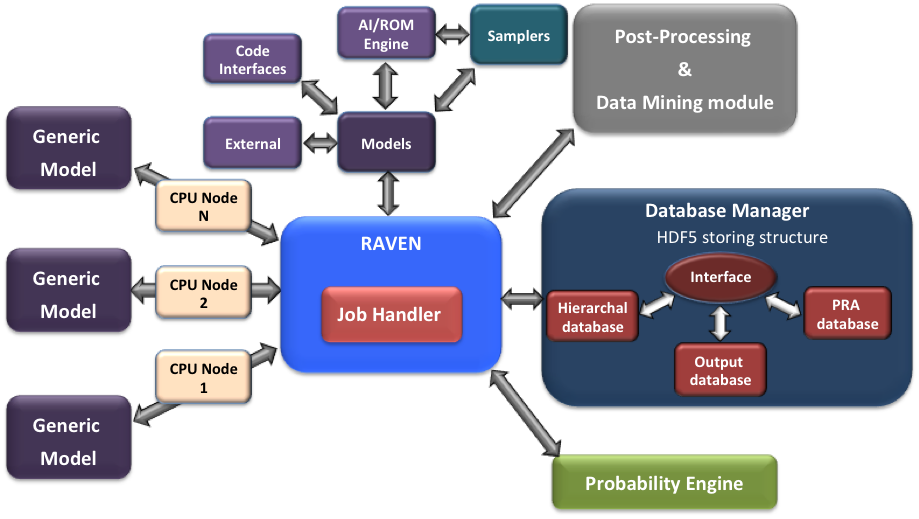
\includegraphics[width=1.0\textwidth]  {pics/RavenFramework.png}
  \caption{RAVEN framework layout}
  \label{fig:RAVENframeworkLayout}
\end{figure}

Hence, RAVEN is coded in $Python$ and is characterized by an object-oriented design. The core of the analysis performable through RAVEN is represented by a set of basic components (objects) the user can combine, in order to create a custom analysis flow. A list of these components and a summary of their most important functionalities are reported as follows:
\begin{itemize}
\item	Distribution: In order to explore the input/output space, RAVEN requires the capability to perturb the input space (initial conditions and/or model coefficients of a system code). The input space is generally characterized by probability distribution functions (PDFs), which might need to be considered when a perturbation is applied. In this respect, a large library of PDFs is available.
\item Sampler: A proper approach to sample the input space is fundamental for the optimization of the computational time. In RAVEN, a ``sampler'' employs a unique perturbation strategy that is applied to the input space of a system. The input space is defined through the connection of uncertain variables and their relative probability distributions. 
\item Model: A model is the representation of a physical system (e.g. Nuclear Power Plant); it is therefore capable of predicting the evolution of a system given a coordinate set in the input space. In addition it can represent an
action on a data in order to extract key features (e.g. Data mining).
\item Reduced Order Model (ROM): The evaluation of the system response, as a function of the coordinates in the input space, is very computationally expensive, especially when brute-force approaches (e.g. Monte Carlo methods) are chosen as the sampling strategy. ROMs are used to lower this cost, reducing the number of needed points and prioritizing the area of the input space that needs to be explored. They can be considered as an artificial representation of the link between the input and output spaces for a particular system. 
\end{itemize}
The list above is not comprehensive of all the RAVEN framework components (visualization and storage infrastructure).
\\ Figure~\ref{fig:RAVENframeworkLayout} shows a schematic representation of the whole framework, highlighting the communication pipes among the different modules and engines. As can be seen, in the figure all the components reported above are schematically shown. In addition the data management, mining and processing modules are shown.

\subsubsection{Distribution}
As already mentioned, the perturbation of the input space, through the initial conditions (parameters) affected by uncertainties, needs to be performed by the proper distribution functions. RAVEN provides, through an interface to the BOOST library, the following variate (truncated and not) distributions: Bernoulli, Binomial, Exponential, Logistic, Lognormal, Normal, Poisson, Triangular, Uniform, Weibull, Gamma, and Beta.
\\The usage of uni-variate distributions for sampling initial conditions is based on the assumption that the uncertain parameters are not correlated with each other. Quite often uncertain parameters are subject to correlations and thus the uni-variate approach is not applicable. This happens when a generic outcome is dependent on different phenomena simultaneously (i.e. the outcome dependency description can not be collapsed to a function of a single variable). RAVEN currently supports both N-dimensional (N-D) PDFs. The user can provide the distribution values on either Cartesian or sparse grid, which determines the interpolation algorithm used in the evaluation of the imported CDF/PDF:
\begin{enumerate}
\item N-Dimensional Spline, for Cartesian grids
\item Inverse weight, for sparse grids
\end{enumerate}
Internally, RAVEN provides the needed N-D differentiation and integration algorithms to compute the PDF from the CDF and vice-versa. 
\\As already mentioned, the sampling methods use the distributions in order to perform probability-weighted perturbations. For example, in the Monte Carlo approach, a random number $\in [0,1]$ is generated (probability threshold) and the CDF, corresponding to that probability, is inverted in order to retrieve the parameter value usable in the simulation. The existence of the inverse for variate distributions is guaranteed by the monotonicity of the CDF. For N-D distributions this condition is not sufficient since the $CDF(X)\longrightarrow [0,1],X \in  R^{N} $ and therefore it could not be a bijective function. From an application point of view, this means the inverse of a N-D CDF is not unique. 
\\As an example, the Figure~\ref{fig:NDDistributionExample} shows a multivariate normal distribution for a pipe failure as function of the pressure and temperature. The plane identifies an isoprobability surface (in this case, a line) that represents a probability threshold of 50 \% in this example.  Hence, the inverse of this CDF is an infinite number of points.
 \\As easily inferable, the standard sampling approach cannot directly be employed. When multivariate distributions are used, RAVEN implements a surface search algorithm for identifying the iso-probability surface location. Once the location of the surface has been found, RAVEN chooses, randomly, one point on it.

\begin{figure}
  \centering
  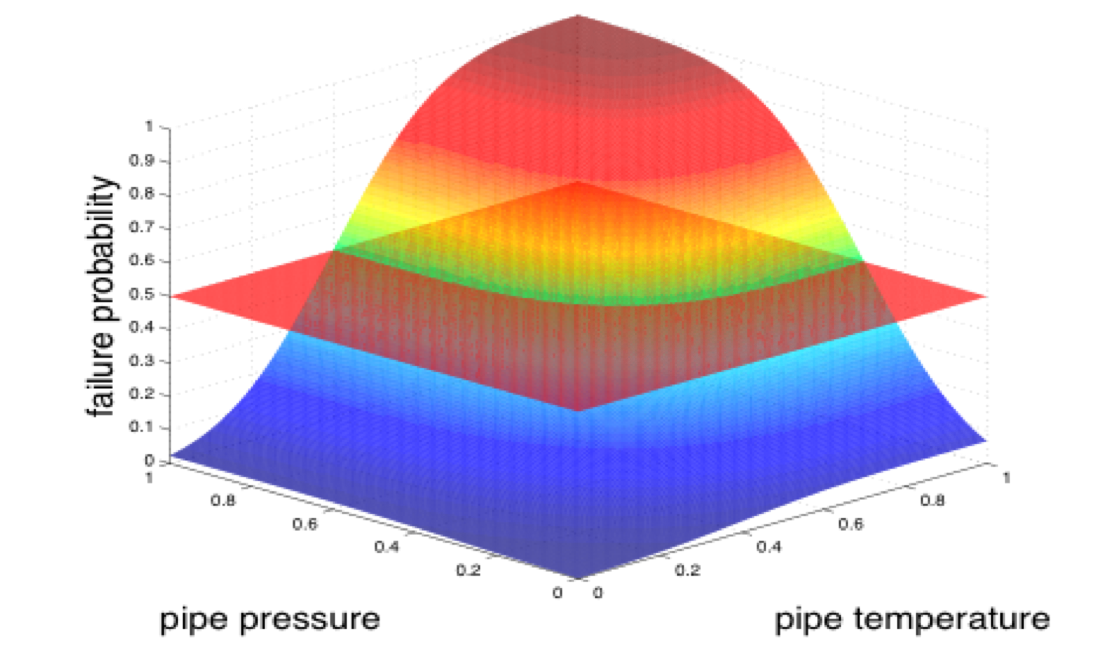
\includegraphics[width=0.5\textwidth]  {pics/NDimensionalDistributionExample.png}
  \caption{2-D CDF, function of pressure and temperature}
  \label{fig:NDDistributionExample}
\end{figure}

\subsubsection{Sampler}

The sampler is probably the most important entity in the RAVEN framework. Indeed, it performs the driving of the specific sampling strategy and, hence, determines the effectiveness of the analysis, from both an accuracy and computational point of view.  The samplers, that are available in RAVEN, can be categorized in three main classes:
\begin{itemize}
 \item Forward
 \item Dynamic Event Tree (DET)
 \item Adaptive
\end{itemize}
\paragraph{Forward Samplers} ~\\ 
The Forward sampler category collects all the strategies that perform the sampling of the input space without exploiting, through dynamic learning approaches, the information made available from the outcomes of calculation previously performed (adaptive sampling) and the common system evolution (patterns) that different sampled calculations can generate in the phase space (dynamic event tree). 
In the RAVEN framework, several different and well-known forward samplers are available:
\begin{itemize}
\item Monte Carlo (MC)
\item Stratified based, whose most known specialization is the Latin Hyper-Cube Sampling (LHS)
\item Grid Based
\item Response Surface Design of Experiment
\item Sparse Grid
\item Factorials
\item Etc.
\end{itemize}
As already mentioned, all these sampling strategies are well known, as well as their properties. Therefore, a detailed investigation of their application is not provided.
%%%%%%%%%%%%%%%%%%%%%%%%%%%%%%%%%%%%%%%%%%%%%%%%%%%%%%%%%%%%%%%%%%%%%%%%%%%%%%%%
\paragraph{Dynamic Event Tree Samplers}~\\
In order to clarify the idea behind the Dynamic Event Tree Sampler currently available in RAVEN, a small overview is needed. 
\\In technological complex systems, as nuclear power plants, an accident scenario begins with an initiating event and then evolves over time through the interaction of dynamics and stochastic events. This mutual action leads to the production of infinitely many different scenarios, which define a continuous dynamic event tree with infinite branches. At each time point, the stochastic variability of the accident outcomes is determined by a multivariate probability distribution. The PRA analysis needs an approximation to this distribution for selected consequence variables. A way to achieve this goal is an Event Tree approach. In dynamic PRA analysis, Conventional Event Tree ~\cite{} sequences are run simultaneously starting from a single initiating event. The branches occur at user specified times and/or when an action is required by the operator and/or the system, creating a deterministic sequence of events based on the time of their occurrence. One of the disadvantages of this method is that the timing/sequencing of events and system dynamics is not explicitly accounted for in the analysis. In order to overcome these limitations a “dynamic” approach is needed. The Dynamic Event Tree (DET) ~\cite{} technique brings several advantages, among which is the fact that it simulates probabilistic system evolution in a way that is consistent with the severe accident model. This leads to a more realistic and mechanistically consistent analysis of the system taken into consideration. The dynamic PRA ~\cite{}, in general, and the Dynamic Event Tree methodologies in particular, are designed to take the timing of events explicitly into account, which can become very important especially when uncertainties in complex phenomena are considered. Hence, the main idea of this methodology is to let a system code determine the pathway of an accident scenario.
\\From an application point of view, a N-D grid is built on the CDF space. A single simulation is spawned and a set of triggers is added to the system code control logic. Every time a trigger gets activated (one of the CDF thresholds in the grid is violated), a new set of simulations (branches) is spawned. Each branch carries its own probability. 
\\Figure \ref{fig:DETschemeExample} shows a practical example. In this particular case, it is assumed that the 
probability failure of a pipe depends on the fluid pressure magnitude. Three probability thresholds are defined on 
the cumulative distribution function. One simulation is spawned (0). As soon as the pressure of the fluid reaches a 
value corresponding to a 33\% probability (CDF), a stop signal is sent and the framework starts two new 
simulations (branches). The branch in which the system evolved to the newer condition (pipe failed, red line) 
carries 33\% of the probability, while the other the complementary amount. The same procedure is repeated at 
point 2.
\\Generally, not all the input space can be explored using a DET approach. For instance, usually the parameters affected by aleatory uncertainty are sampled using a dynamic event tree approach, while the ones characterized by epistemic uncertainty are sampled through ``forward'' sampling strategies. 
\\As already mentioned, this strategy requires a tight interaction between the system code and the sampling driver (i.e., RAVEN framework). In addition, the system code must have a control logic capability (i.e. trigger system). For these reasons, the application of this sampling approach to a generic code needs a larger effort when compared to the other Samplers available in RAVEN. Currently, the DET is fully available for the thermal-hydraulic codes RELAP-7 and RELAP5-3D.
\\In the RAVEN framework, several different DET-based samplers are available:
\begin{itemize}
\item Dynamic Event Tree (aleatory sampling);
\item Hybrid Dynamic Event Tree (aleatory and epistemic sampling);
\item Adaptive Dynamic Event Tree (goal-oriented sampling for aleatory sampling);
\item Adaptive Hybrid Dynamic Event Tree (goal-oriented sampling for aleatory and epistemic sampling).
\end{itemize}

\begin{figure}
  \centering
  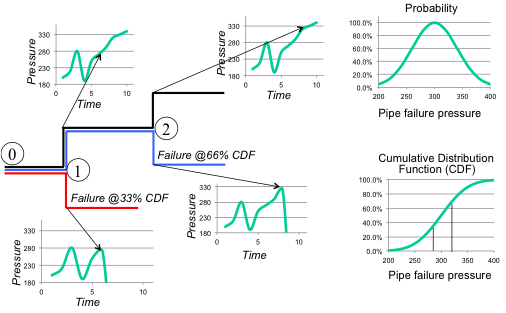
\includegraphics[width=0.7\textwidth]  {pics/DETscheme.png}
  \caption{Dynamic Event Tree simulation pattern}
  \label{fig:DETschemeExample}
\end{figure}

%%%%%%%%%%%%%%%%%%%%%%%%%%%%%%%%%%%%%%%%%%%%%%%%%%%%%%%%%%%%%%%%%%%%%%%%%%%%%%%%
\paragraph{Adaptive Samplers}~\\ 
A key feature available within RAVEN is the possibility to perform smart sampling (also known as adaptive sampling) as an alternative to classical ``forward'' techniques.
\\The motivation is that nuclear simulations are often computationally expensive, time-consuming, and high dimensional with respect to the number of input parameters. Thus, exploring the space of all possible simulation outcomes is unfeasible using finite computing resources. During simulation-based probabilistic risk analysis, it is important to discover the relationship between a potentially large number of input parameters and the output of a simulation using as few simulation trials as possible. 
\\This is a typical context for performing adaptive sampling where a few observations are obtained from the simulation, a reduced order model (ROM) is built to represent the simulation space, and new samples are selected based on the model constructed. The ROM is then updated based on the simulation results of the sampled points. In this way, it is attempted to gain the most information possible with a small number of carefully selected sampled points, limiting the number of expensive trials needed to understand features of the system space.
\\In the RAVEN framework, several different adaptive samplers are available:
\begin{itemize}
\item Limit Surface Search;
\item Adaptive Dynamic Event Tree;
\item Adaptive Hybrid Dynamic Event Tree ;
\item Adaptive Sparse Grid;
\item Adaptive Sobol Decomposition.
\end{itemize}

\subsubsection{Models} 
The Model entity, in the RAVEN environment, represents a ``connection pipeline'' between the input and the output space. The RAVEN framework does not own any physical model (i.e. it does not posses the equations needed to simulate a generic physical system, such as Navier-Stocks equations, Maxwell equations, etc.), but implements Application Program Interfaces (APIs) by which any generic model can be integrated and interrogated. The RAVEN framework provides APIs for four different model categories: Codes, Externals, Post-Processors (PPs) and Reduced Order Models (ROMs). In the following paragraphs, a brief explanation of each of this Model categories is reported. 
\paragraph{Code} ~\\ 
The \textit{Code} model represents the communication pipe between the RAVEN framework and any system and physical code. The communication between RAVEN and any driven code is performed through the implementation of interfaces directly operated by the framework. 
\\The procedure of coupling a new code/application with RAVEN is a straightforward process. The coupling is performed through a \textit{Python}  interface that interprets the information coming from RAVEN and translates them to the input of the driven code. The coupling procedure does not require modifying RAVEN itself. Instead, the developer creates a new \textit{Python} interface that is going to be embedded in RAVEN at run-time (no need to introduce hard-coded coupling statements).  This interface needs to be placed in a folder (whatever name) located in (see figure~\ref{fig:CodeInterfaceLocation}):
\begin{lstlisting}[language=bash]
 path/to/raven/distribution/raven/framework/CodeInterfaces/
\end{lstlisting}

\begin{figure}
  \centering
  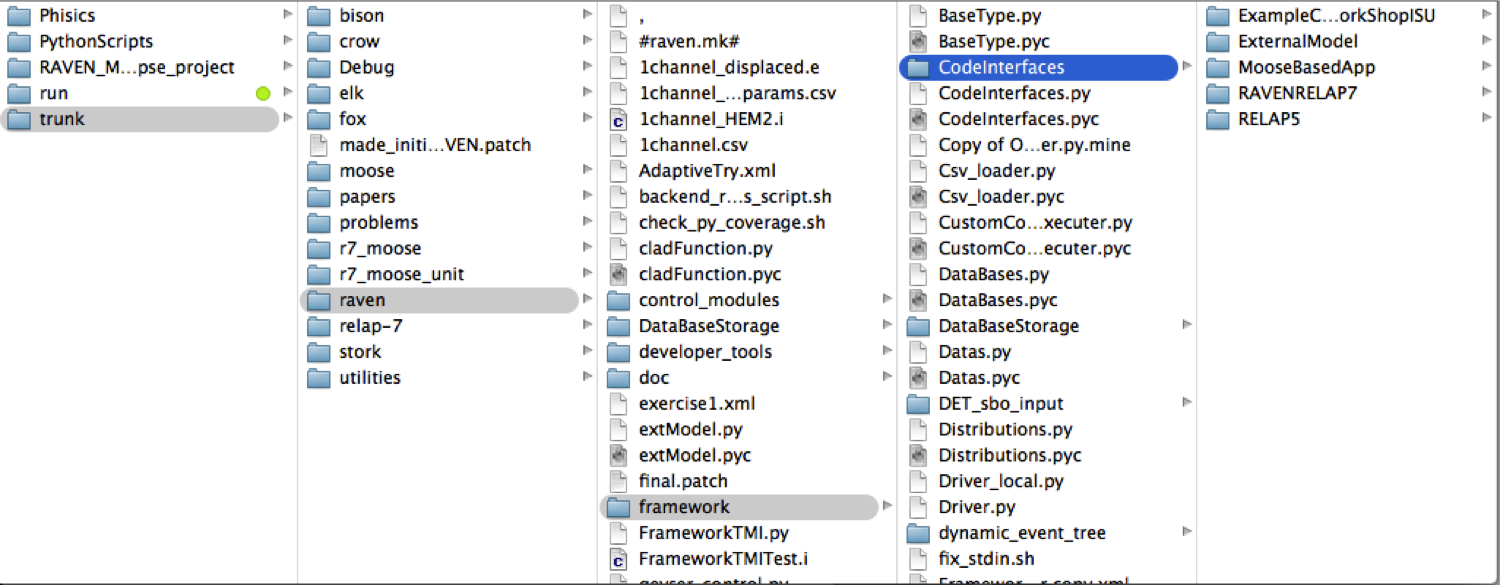
\includegraphics[width=0.8\textwidth]  {pics/CodeInterfaceLocation.png}
  \caption{Code Interface Location}
  \label{fig:CodeInterfaceLocation}
\end{figure}
At the initialization stage, RAVEN imports all the Interfaces that are contained in this directory and performs some preliminary cross-checks. 
\\ If the coupled code is parallelized and/or multi-threaded, RAVEN is going to manage the system in order to optimize the computational resources in both workstations and High Performance Computing systems.
\\Currently, RAVEN has APIs for RELAP5-3D, RELAP-7, any MOOSE-based application, SASS and Modelica.
\paragraph{External Model} ~\\
The External model allows the user to create, in a \textit{Python} file (imported, at run-time, in the RAVEN framework), its own model (e.g. set of equations representing a physical model, connection to another code, control logic, etc.). This model will be interpreted/used by the framework and, at run-time, will become part of RAVEN itself.
\paragraph{Post-Processor} ~\\
The Post-Processor model represents the container of all the post-processing capabilities in the RAVEN code. This model is aimed to process the data (for example, derived from the sampling of a physical code) in order to identify representative Figure of Merits. This system has  been designed and, presently, is under heavy development by the whole RAVEN team.  Currently, the following post-processors are available:
\begin{itemize}
 \item \textit{Basic Statistics}, container of the algorithms to compute many of the most important statistical quantities. This post-processor is able to compute mean, sigma/variance, variation coefficient, skewness, kurtosis, median, percentiles and all the principal matrix quantities such as covariance, sensitivity (either leas-squared and variance weighted) and correlation matrices;
 \item \textit{Comparison Statistics}, aimed to employ validation and verification metrics;
 \item \textit{Limit Surface}, aimed to compute the limit surface in the input space (i.e. the hyper-surface that represents the boundary between the failure/success of the system);
 \item \textit{Limit Surface Integral}, intended to compute the integral of the limit surface that corresponds to the probability of failure;
  \item \textit{Safest Point}, provides the coordinates of the farthest point from the limit surface that is given as an input. The safest point coordinates are expected values of the coordinates of the farthest points from the limit surface in the space of the ``controllable'' variables based on the probability distributions of the ``non-controllable'' variables. The term ``controllable'' identifies those variables that are under control during the system operation, while the ``non-controllable'' variables are stochastic parameters affecting the system behavior randomly;
 \item \textit{External Post-Processor}, user-defined post-processor;
 \item \textit{Topological Decomposition}, aimed to compute an approximated hierarchical Morse-Smale complex which will add two columns to a data-set, performing a topological decomposition of such data-set;
 \item \textit{Data Mining}, container of all the RAVEN data mining, clustering and dimensionality reduction techniques aimed to identify dominant and common patterns in high-dimensionality data.
\end{itemize}
\paragraph{Reduced Order Model} ~\\
 As briefly mentioned, a ROM is a mathematical representation of a system, used to predict a selected output space of a physical system. 
The ``training'' is a process that uses sampling of the physical model to improve the prediction capability (capability to predict the status of the system given a realization of the input space) of the ROM. More specifically, in RAVEN the Reduced Order Model is trained to emulate a high fidelity numerical representation (system codes) of the physical system. Two general characteristics of these models can be generally assumed (even if exceptions are possible):
\begin{enumerate}
   \item The higher the number of realizations in the training sets, the higher is the accuracy of the prediction performed by the reduced order model. This statement is true for most of the cases although some ROMs might be subject to the over-fitting issues. The over-fitting phenomenon is not discussed here, since its occurrence is highly dependent on the algorithm type, (and there is large number of ROM options available in RAVEN). Every time the user chooses a particular reduced order model algorithm to use, he should consult the relative literature;
   \item The smaller the size of the input domain with respect to the variability of the system response, the more likely the surrogate model will be able to represent the system output space.
\end{enumerate}
In most of the cases of interest, the information that is sought is related to defining the failure boundaries of a system with respect to perturbations in the input space. For this reason, in the development of RAVEN, it has been given priority to the introduction of a class of supervised learning algorithms, which are usually referred to as classifiers. A classifier is a reduced order model that is capable of representing the system behavior through a binary response (failure/success). 
\\The first class of classifier introduced has been the Support Vector Machines (SVMs) [reference] with several different kernels (polynomial of arbitrary integer order, radial basis function kernel, sigmoid) followed by a nearest-neighbor based classification using a K-D tree search algorithm. Currently, RAVEN supports around 40 different ROM methodologies. All these supervised learning algorithms have been imported via an API from the scikit-learn [reference] library. In addition, the N-Dimensional spline and the inverse weight methods, that are currently available for the interpolation of N-Dimensional PDF/CDF, can also be used as ROMs.
\subsubsection{Simulation Environment} 
RAVEN is perceived by the user as a pool of tools and data. Any action in which the tools are applied to the data is considered a calculation ``step'' in the RAVEN environment. Simplistically, a ``step'' can be seen as a \textbf{transfer function} between the input and output space through a Model (e.g. Code, External, ROM or Post-Processor). One of the most important step in the RAVEN framework is called ``multi-run'', that is aimed to handle calculations that involve multiple runs of a driven code (sampling strategies). Firstly, the RAVEN input file associates the variables to a set of PDFs and to a sampling strategy. The ``multi-run'' step is used to perform several runs in a block of a model (e.g. in a MC sampling).
\begin{figure}[ht]
  \centering
  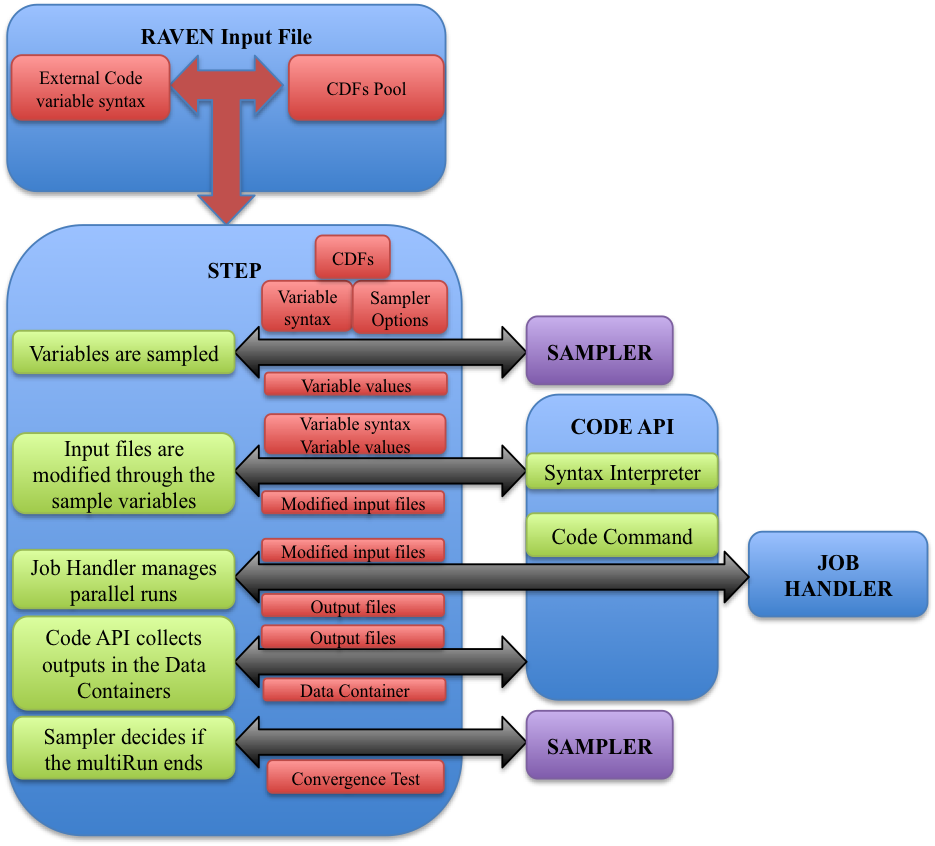
\includegraphics[width=0.8\textwidth]  {pics/MultiRunCalculationFlow.png}
  \caption{Calculation flow for a multi-run sampling}
  \label{fig:multiRun}
\end{figure}
At the beginning of each sub sequential run, the sampler provides the new values of the variables to be perturbed. The code API places those values in the input file. At this point, the code API generates the run command and asks to be queued by the job handler. The job handler manages the parallel execution of as many runs as possible within a user prescribed range and communicates with the step controller when a new set of output files are ready to be processed. The code API receives the new input files and collects the data in the RAVEN internal format. The sampler is queried to assess if the sequence of runs is ended, if not, the step controller asks for a new set of values from the sampler and the sequence is restarted as described in Figure~\ref{fig:multiRun}. 
The job handler is currently capable to run different run instances of the code in parallel and can also handle codes that are multi-threaded or using any form of parallel implementation.
RAVEN also has the capability to plot the simulation outcomes while the set of sampling is performed and to store the data for later recovery.